\chapter{Fotosíntesis y autotrofía}\label{ch:b1:photosynthesis}

Todos los gramos de carbono del conejo, del roble, del lector y de esta
página fueron alguna vez dióxido de carbono del aire, y una \omterm{def:b1:flowering-plant-organization:organs}{hoja} --- o un
alga, o una cianobacteria --- los fijó en azúcar con la energía de la luz
solar. La reacción, seis $\mathrm{CO_2}$ y seis aguas hasta una glucosa y
seis oxígenos, va cuesta arriba en \qty{2870}{kJ/mol}; una \omterm{def:b1:flowering-plant-organization:organs}{hoja} la hace
funcionar escindiendo agua con luz, almacenando los electrones en NADPH y la
energía en \omterm{def:b1:water-small-molecules:atp}{ATP}, y gastando ambos en un ciclo que construye azúcar. Este
capítulo describe el \omterm{def:b1:photosynthesis:chloroplast}{cloroplasto}, los pigmentos y las \omterm{prop:b1:photosynthesis:lightreactions}{reacciones luminosas}
que fabrican \omterm{def:b1:water-small-molecules:atp}{ATP} y NADPH, el \omterm{def:b1:photosynthesis:fixation}{ciclo de Calvin} que fija el carbono, la fuga
llamada fotorrespiración y los dos diseños que la cierran, y qué es la
\omterm{def:b1:photosynthesis:autotrophy}{autotrofía} en general.

\section{El cloroplasto y sus pigmentos}

\begin{definition}[Cloroplasto]\label{def:b1:photosynthesis:chloroplast}
El \emph{cloroplasto}\index{cloroplasto} es un orgánulo con forma de lente,
de \qtyrange{3}{10}{\micro m} de largo, delimitado por dos membranas de
envoltura; su interior, el \emph{estroma}\index{estroma}, contiene las
\omterm{def:b1:enzymes:enzyme}{enzimas} de la fijación del carbono, granos de \omterm{def:b1:carbohydrates:polysaccharide}{almidón}, ribosomas y un \omterm{def:b1:nucleic-acids:chain}{ADN}
circular; dentro del estroma, un tercer sistema de membranas, los
\emph{tilacoides}\index{tilacoide}, forma sáculos aplanados apilados en
\emph{granas} y conectados por lamelas, que encierran una \emph{luz
tilacoidal} continua. Las \omterm{prop:b1:photosynthesis:lightreactions}{reacciones luminosas} ocurren en la membrana
tilacoidal; la fijación del carbono, en el estroma. Una \omterm{def:b1:cell-unit-of-life:cell}{célula} de \omterm{def:b1:flowering-plant-organization:organs}{hoja}
contiene de \qtyrange{20}{100}{} \omterm{def:b1:eukaryotic-cell:plastid}{cloroplastos}; un milímetro cuadrado de
\omterm{def:b1:flowering-plant-organization:organs}{hoja}, medio millón.
\end{definition}

\begin{omfigure}
\begin{tikzpicture}
  \node[anchor=south west, inner sep=0] (img) at (0,0)
    {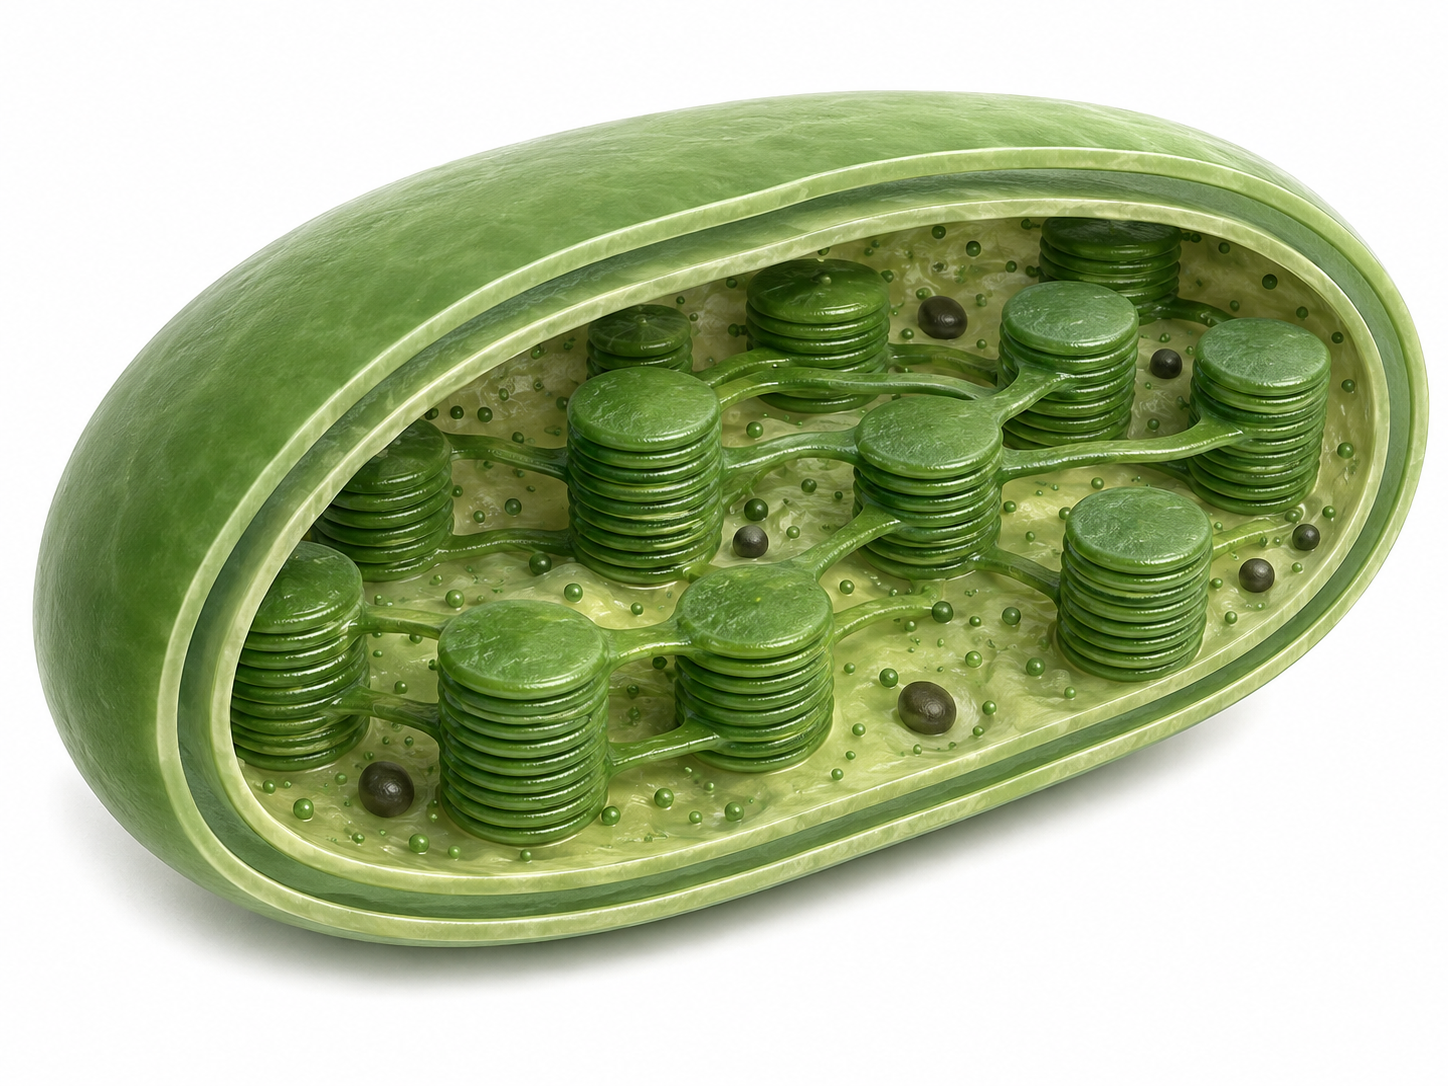
\includegraphics[width=0.56\linewidth]{images/book3/ai/fig-chloroplast-cutaway.png}};
  \begin{scope}[x={(img.south east)}, y={(img.north west)},
      every node/.style={font=\small}]
    \draw[omDef, thick] (0.12,0.50) -- (-0.03,0.66) node[left, align=right] {dos membranas\\ de envoltura};
    \draw[omDef, thick] (0.48,0.60) -- (0.48,1.08) node[above] {grana: una pila de tilacoides};
    \draw[omDef, thick] (0.62,0.52) -- (1.03,0.62) node[right] {lamela del estroma};
    \draw[omDef, thick] (0.35,0.24) -- (-0.03,0.16) node[left] {estroma};
    \draw[omDef, thick] (0.86,0.50) -- (1.03,0.40) node[right] {grano de almidón};
  \end{scope}
\end{tikzpicture}

{\small Un \omterm{def:b1:photosynthesis:chloroplast}{cloroplasto} abierto. Dos membranas de envoltura en torno al
\omterm{def:b1:photosynthesis:chloroplast}{estroma}; dentro, pilas de \omterm{def:b1:photosynthesis:chloroplast}{tilacoides} (granas) conectadas por lamelas y que
encierran una sola luz. La luz se capta en la membrana tilacoidal y el
azúcar se fabrica en el \omterm{def:b1:photosynthesis:chloroplast}{estroma}.}
\end{omfigure}

\begin{definition}[Pigmentos fotosintéticos]\label{def:b1:photosynthesis:pigments}
Las \emph{clorofilas}\index{clorofila} $a$ y $b$ son anillos de porfirina en
torno a un átomo de magnesio, con una cola hidrófoba larga que las ancla en
la membrana tilacoidal; absorben luz azul (\qtyrange{430}{450}{nm}) y roja
(\qtyrange{640}{680}{nm}) y reflejan el verde. Los
\emph{carotenoides}\index{carotenoide} (\omterm{def:b1:lipids:steroids}{isoprenoides}, \cref{ch:b1:lipids})
absorben luz azul verdosa y transmiten la energía a la clorofila, y la
protegen amortiguando el exceso de excitación. Unos cientos de moléculas de
pigmento, sostenidas por \omterm{def:b1:proteins:peptide}{proteínas} como una \emph{antena} (complejo captador
de luz), canalizan la energía de cada fotón absorbido hacia una pareja
especial de moléculas de clorofila $a$, el \emph{centro de reacción}, donde
se convierte en química.
\end{definition}

\begin{omfigure}
\begin{tikzpicture}
\begin{axis}[
  width=0.88\linewidth, height=6.2cm,
  axis x line=bottom, axis y line=left,
  xmin=400, xmax=720, ymin=0, ymax=1.1,
  xlabel={longitud de onda (\unit{nm})}, ylabel={absorción, o velocidad (relativa)},
  xlabel style={font=\small, at={(axis description cs:0.5,-0.12)}, anchor=north},
  ylabel style={font=\small},
  tick label style={font=\small}, xtick={400,450,500,550,600,650,700}, ytick={0,0.5,1},
  legend style={font=\small, at={(0.5,0.98)}, anchor=north, draw=none},
  clip=false,
]
\addplot[very thick, omDef, domain=400:720, samples=160] {exp(-((x-430)/18)^2) + 0.85*exp(-((x-662)/14)^2) + 0.05};
\addlegendentry{absorción de la clorofila $a$}
\addplot[very thick, omExo, domain=400:720, samples=160] {0.7*exp(-((x-455)/20)^2) + 0.5*exp(-((x-645)/14)^2) + 0.05};
\addlegendentry{absorción de la clorofila $b$}
\addplot[very thick, omProp, domain=400:720, samples=160] {0.75*exp(-((x-470)/25)^2) + 0.05};
\addlegendentry{absorción de los carotenoides}
\addplot[very thick, dashed, omThm, domain=400:720, samples=160] {0.9*exp(-((x-440)/30)^2) + 0.35*exp(-((x-520)/50)^2) + 0.85*exp(-((x-660)/22)^2) + 0.1};
\addlegendentry{espectro de acción: velocidad de liberación de $\mathrm{O_2}$}
\end{axis}
\end{tikzpicture}

{\small Espectros de absorción de las tres clases de pigmento y espectro de
acción de la fotosíntesis (la velocidad de liberación de oxígeno a cada
longitud de onda). El espectro de acción sigue a las \omterm{def:b1:photosynthesis:pigments}{clorofilas}, y los
\omterm{def:b1:photosynthesis:pigments}{carotenoides} lo rellenan en el azul verdoso: todo pigmento que absorbe
contribuye.}
\end{omfigure}

\begin{proposition}[El espectro de acción sigue a los pigmentos]\label{prop:b1:photosynthesis:engelmann}
La fotosíntesis la impulsa la luz que absorben los pigmentos: es más rápida
con luz roja y azul y más débil con luz verde.
\end{proposition}
\begin{proof}[Evidencia]
Engelmann (1882) colocó un filamento de alga a través de un espectro
proyectado bajo su microscopio y añadió bacterias que buscan oxígeno: se
reunieron donde caía la luz roja y la azul, no en la verde (recordado del
volumen de bachillerato). Medida con un electrodo de oxígeno, la velocidad
en cada longitud de onda da el espectro de acción anterior, que sigue a la
absorción de las \omterm{def:b1:photosynthesis:pigments}{clorofilas}; el exceso en el azul verdoso es la contribución
de los \omterm{def:b1:photosynthesis:pigments}{carotenoides}, lo que muestra que transmiten su energía.
\end{proof}

\section{Las reacciones luminosas}

\begin{proposition}[Qué hacen las reacciones luminosas]\label{prop:b1:photosynthesis:lightreactions}
\index{reacciones luminosas}
En la membrana tilacoidal, la energía de la luz se usa para llevar
electrones desde el agua hasta el $\mathrm{NADP^+}$ --- cuesta arriba,
contra una diferencia de potencial redox de \qty{1.1}{V} --- y para bombear
protones hacia la luz tilacoidal:
\[
2\,\mathrm{H_2O} + 2\,\mathrm{NADP^+} + 3\,\mathrm{ADP} + 3\,\mathrm{P_i}
\xrightarrow{\ 8\ \text{fotones}\ }
\mathrm{O_2} + 2\,\mathrm{NADPH} + 2\,\mathrm{H^+} + 3\,\mathrm{ATP} .
\]
El oxígeno liberado es el oxígeno del agua, no el del dióxido de carbono; el
NADPH lleva el poder reductor y el \omterm{def:b1:water-small-molecules:atp}{ATP} la energía que gastará el \omterm{def:b1:photosynthesis:fixation}{ciclo de
Calvin}.
\end{proposition}
\begin{proof}[Evidencia]
Hill (1937) mostró que \omterm{def:b1:eukaryotic-cell:plastid}{cloroplastos} aislados iluminados liberan oxígeno en
ausencia de $\mathrm{CO_2}$ si hay presente un aceptor artificial de
electrones: la escisión del agua es separable de la fijación del carbono.
Ruben y Kamen (1941) dieron a unas algas agua marcada con oxígeno pesado y
encontraron la marca en el $\mathrm{O_2}$ liberado, y no cuando la marca
estaba en el $\mathrm{CO_2}$. Emerson (1957) descubrió que la luz roja de
\qty{700}{nm}, casi inútil por sí sola, y la luz de \qty{680}{nm} juntas
daban más que la suma de sus velocidades por separado: dos \omterm{def:b1:photosynthesis:zscheme}{fotosistemas} con
pigmentos distintos debían trabajar en serie.
\end{proof}

\begin{definition}[Fotosistemas y el esquema Z]\label{def:b1:photosynthesis:zscheme}
\index{fotosistema}\index{esquema Z}
En la membrana tilacoidal hay dos \emph{fotosistemas}. En el
\emph{fotosistema II} (PSII, centro de reacción P680) un fotón absorbido
eleva un electrón de la pareja especial a una energía alta; el electrón sale
y el P680 oxidado, el oxidante biológico más fuerte, toma un electrón del
agua: un agregado de manganeso escinde dos moléculas de agua en
$\mathrm{O_2}$, cuatro protones (liberados a la luz tilacoidal) y cuatro
electrones, de fotón en fotón. El electrón desciende por una \emph{cadena de
transporte de electrones} --- plastoquinona, el \emph{complejo citocromo
$b_6f$}, plastocianina --- y la energía que pierde bombea protones a la luz.
En el \emph{fotosistema I} (PSI, P700) un segundo fotón lo eleva de nuevo,
hasta un potencial lo bastante bajo para reducir la ferredoxina y después el
$\mathrm{NADP^+}$ a NADPH. Dibujado en una escala de potencial redox, el
camino es una Z: dos ascensos por la luz, dos descensos por la química.
\end{definition}

\begin{omfigure}
\begin{tikzpicture}[font=\footnotesize, >=Stealth, line cap=round,
  st/.style={draw, thick, rounded corners=2pt, inner sep=2pt}]
  % redox potential axis (vertical, more negative up)
  \draw[->, thick] (0,0) -- (0,6.4) node[above, font=\small] {potencial redox $E'_0$ (V)};
  \foreach \y/\l in {0.4/{$+1.0$}, 1.9/{$+0.5$}, 3.4/{$0$}, 4.9/{$-0.5$}, 6.0/{$-0.9$}} { \draw (-0.1,\y) -- (0.1,\y) node[left, xshift=-4pt] {\l}; }
  % PSII
  \node[st, fill=omDef!15] (h2o) at (1.7,1.0) {$\mathrm{H_2O}$};
  \node[st, fill=omDef!25] (p680) at (2.9,0.35) {P680};
  \node[st, fill=omDef!25] (p680s) at (2.9,5.7) {P680*};
  \draw[->, thick] (h2o) -- (p680);
  \node[anchor=west, font=\scriptsize] at (3.5,0.35) {$\to \mathrm{O_2} + 4\,\mathrm{H^+}$ hacia la luz};
  \draw[->, very thick, omProp] (p680) -- (p680s) node[pos=0.45, right, align=left] {fotón\\ (\qty{680}{nm})};
  % chain
  \node[st, fill=omThm!15] (pq) at (4.2,4.4) {PQ};
  \node[st, fill=omThm!15] (b6f) at (5.4,3.6) {cit $b_6f$};
  \node[st, fill=omThm!15] (pc) at (6.5,2.8) {PC};
  \draw[->, thick] (p680s) -- (pq); \draw[->, thick] (pq) -- (b6f); \draw[->, thick] (b6f) -- (pc);
  \node[anchor=south west, align=left, font=\scriptsize, omThm] at (4.75,4.15) {$\mathrm{H^+}$ bombeados\\ hacia la luz};
  % PSI
  \node[st, fill=omExo!25] (p700) at (7.7,2.3) {P700};
  \node[st, fill=omExo!25] (p700s) at (7.7,6.0) {P700*};
  \draw[->, thick] (pc) -- (p700);
  \draw[->, very thick, omProp] (p700) -- (p700s) node[pos=0.45, right, align=left] {fotón\\ (\qty{700}{nm})};
  \node[st, fill=omThm!15] (fd) at (9.1,5.2) {Fd};
  \node[st, fill=omExo!15] (nadp) at (10.5,4.6) {NADPH};
  \draw[->, thick] (p700s) -- (fd); \draw[->, thick] (fd) -- (nadp);
  \node[anchor=north, font=\scriptsize] at (10.5,4.3) {$E'_0 = \qty{-0.32}{V}$};
  % cyclic flow
  \draw[->, thick, dashed, gray] (fd) .. controls (7.2,5.5) and (4.4,5.5) .. (pq.north);
  \node[gray, font=\scriptsize, anchor=south] at (5.6,5.45) {flujo cíclico (solo ATP)};
\end{tikzpicture}

{\small El \omterm{def:b1:photosynthesis:zscheme}{esquema Z}. Los electrones que P680 toma del agua los eleva un
fotón, descienden por una cadena que bombea protones, los eleva de nuevo
P700 y terminan en el NADPH. El eje vertical es el potencial redox, más
negativo hacia arriba: la luz asciende, la química desciende.}
\end{omfigure}

\begin{theorem}[Síntesis quimiosmótica de ATP]\label{thm:b1:photosynthesis:chemiosmosis}
\index{quimiosmosis}\index{ATP sintasa}
Los protones liberados por la escisión del agua y bombeados por el complejo
citocromo $b_6f$ se acumulan en la luz tilacoidal, que con luz baja a pH 5
mientras el \omterm{def:b1:photosynthesis:chloroplast}{estroma} sube a pH 8: una diferencia de tres unidades, una fuerza
protón-motriz de unos \qty{0.18}{V}, equivalente a \qty{17}{kJ} por mol de
protones. La \emph{\omterm{thm:b1:photosynthesis:chemiosmosis}{ATP sintasa}}, un motor rotatorio que atraviesa la
membrana tilacoidal, deja que los protones vuelvan al \omterm{def:b1:photosynthesis:chloroplast}{estroma} y usa la
energía para fosforilar ADP: unos \qty{4}{H^+} por \omterm{def:b1:water-small-molecules:atp}{ATP}. El transporte de
electrones y la síntesis de \omterm{def:b1:water-small-molecules:atp}{ATP} están acoplados únicamente a través de ese
gradiente (teoría quimiosmótica de Mitchell, 1961).
\end{theorem}
\begin{proof}[Evidencia]
Jagendorf (1966) mantuvo \omterm{def:b1:photosynthesis:chloroplast}{tilacoides} en la oscuridad en un baño ácido (pH 4)
hasta que su luz interna se acidificó, y los transfirió después de golpe a
pH 8 con ADP y fosfato: se fabricó \omterm{def:b1:water-small-molecules:atp}{ATP} en la oscuridad, solo a partir del
gradiente. Los desacoplantes --- ácidos débiles liposolubles que llevan
protones a través de las membranas --- suprimen la síntesis de \omterm{def:b1:water-small-molecules:atp}{ATP} mientras
el transporte de electrones y la liberación de oxígeno continúan, e incluso
se aceleran. La \omterm{thm:b1:photosynthesis:chemiosmosis}{ATP sintasa} aislada y reconstituida en vesículas
artificiales fabrica \omterm{def:b1:water-small-molecules:atp}{ATP} cuando se le impone un gradiente de pH, e hidroliza
\omterm{def:b1:water-small-molecules:atp}{ATP} para bombear protones cuando no lo hay. Desde entonces se ha observado
directamente la rotación de la \omterm{def:b1:enzymes:enzyme}{enzima}, molécula a molécula, al microscopio.
\end{proof}

\begin{example}[Flujo cíclico y no cíclico]\label{ex:b1:photosynthesis:cyclic}
El camino lineal del agua al NADPH da, por cada $\mathrm{O_2}$, dos NADPH y
unos tres \omterm{def:b1:water-small-molecules:atp}{ATP}; el \omterm{def:b1:photosynthesis:fixation}{ciclo de Calvin} necesita exactamente una proporción de
tres \omterm{def:b1:water-small-molecules:atp}{ATP} por dos NADPH, y los demás trabajos del \omterm{def:b1:photosynthesis:chloroplast}{cloroplasto} necesitan más
\omterm{def:b1:water-small-molecules:atp}{ATP}. Cuando escasea el \omterm{def:b1:water-small-molecules:atp}{ATP}, los electrones de la ferredoxina vuelven a la
plastoquinona en vez de ir al $\mathrm{NADP^+}$ (\emph{fotofosforilación
cíclica}): el PSI solo, bombeando protones y fabricando \omterm{def:b1:water-small-molecules:atp}{ATP} sin oxígeno ni
NADPH. Los dos modos se equilibran según la demanda.
\end{example}

\section{El ciclo de Calvin}

\begin{definition}[Fijación del carbono]\label{def:b1:photosynthesis:fixation}
\index{ciclo de Calvin}\index{RuBisCO}
El \emph{ciclo de Calvin} del \omterm{def:b1:photosynthesis:chloroplast}{estroma} fija el $\mathrm{CO_2}$ en azúcar en
tres etapas. \emph{Fijación}: la \emph{RuBisCO} (ribulosa bisfosfato
carboxilasa/oxigenasa) añade $\mathrm{CO_2}$ a la ribulosa-1,5-bisfosfato
(RuBP, cinco carbonos), y el producto de seis carbonos se escinde al
instante en dos moléculas de 3-fosfoglicerato (3-PGA, tres carbonos).
\emph{Reducción}: cada 3-PGA se fosforila con \omterm{def:b1:water-small-molecules:atp}{ATP} y se reduce con NADPH a
gliceraldehído-3-fosfato (G3P), el primer azúcar. \emph{Regeneración}: cinco
de cada seis G3P se reorganizan, a costa de \omterm{def:b1:water-small-molecules:atp}{ATP}, para volver a dar tres RuBP,
y un G3P abandona el ciclo como producto neto. La estequiometría para un G3P
(tres carbonos) es
\[
3\,\mathrm{CO_2} + 9\,\mathrm{ATP} + 6\,\mathrm{NADPH} + 6\,\mathrm{H^+}
\to \text{G3P} + 9\,\mathrm{ADP} + 8\,\mathrm{P_i} + 6\,\mathrm{NADP^+} ;
\]
dos G3P dan una glucosa: \qty{18}{} \omterm{def:b1:water-small-molecules:atp}{ATP} y \qty{12}{NADPH} por glucosa.
\end{definition}

\begin{omfigure}
\begin{tikzpicture}[font=\footnotesize, >=Stealth, line cap=round,
  box/.style={draw, thick, rounded corners=3pt, minimum height=8mm, align=center, fill=white}]
  \node[box, fill=omDef!15] (rubp) at (0,2.6) {3 RuBP\\ ($3\times$ C5)};
  \node[box, fill=omDef!15] (pga) at (5.0,2.6) {6 3-PGA\\ ($6\times$ C3)};
  \node[box, fill=omDef!15] (g3p) at (5.0,-0.4) {6 G3P\\ ($6\times$ C3)};
  \node[box, fill=omExo!20] (out) at (9.2,-0.4) {sale 1 G3P\\ (ganancia neta: 3 C)};
  \draw[->, very thick, omThm] (rubp) -- (pga) node[midway, above, align=center] {fijación (RuBisCO)\\ $+\,3\,\mathrm{CO_2}$};
  \draw[->, very thick, omThm] (pga) -- (g3p) node[midway, right, align=left] {reducción\\ $6\,\mathrm{ATP}$, $6\,\mathrm{NADPH}$};
  \draw[->, very thick, omThm] (g3p) -- (out);
  \draw[->, very thick, omThm] (g3p) -| (rubp);
  \node[anchor=north, align=center, omThm] at (2.4,-0.95) {regeneración: 5 G3P $\to$ 3 RuBP\\ $3\,\mathrm{ATP}$};
  \node[anchor=north, align=center, gray] at (4.6,-1.7) {por vuelta (tres $\mathrm{CO_2}$): 9 ATP, 6 NADPH, un G3P ganado\\ dos vueltas: una glucosa, 18 ATP, 12 NADPH};
\end{tikzpicture}

{\small El \omterm{def:b1:photosynthesis:fixation}{ciclo de Calvin} para tres moléculas de $\mathrm{CO_2}$: tres RuBP
fijados en seis 3-PGA, reducidos a seis G3P, de los cuales uno sale y cinco
regeneran los tres RuBP. El carbono se conserva en cada paso
($15 + 3 = 18 = 3 + 15$).}
\end{omfigure}

\begin{proposition}[La evidencia de Calvin]\label{prop:b1:photosynthesis:calvin}
El primer producto estable de la fijación del $\mathrm{CO_2}$ es el
3-fosfoglicerato, y el aceptor es la ribulosa bisfosfato.
\end{proposition}
\begin{proof}[Evidencia]
Calvin y Benson (1948--1954) iluminaron algas en un matraz plano (la
``piruleta''), inyectaron $\mathrm{^{14}CO_2}$ y mataron muestras en alcohol
hirviendo al cabo de unos segundos; la cromatografía en papel bidimensional
y la autorradiografía mostraron dónde estaba la marca. A los cinco segundos
casi toda estaba en el 3-PGA; con exposiciones más largas se repartía por
los azúcares fosforilados y después por la sacarosa y el \omterm{def:b1:carbohydrates:polysaccharide}{almidón}. Al retirar
de golpe el $\mathrm{CO_2}$, la RuBP se acumulaba y el 3-PGA caía; al apagar
la luz, el 3-PGA se acumulaba y la RuBP caía; luego la RuBP es el aceptor
que consume la fijación, y el 3-PGA el producto que consumen el \omterm{def:b1:water-small-molecules:atp}{ATP} y el
NADPH de la luz.
\end{proof}

\begin{omfigure}
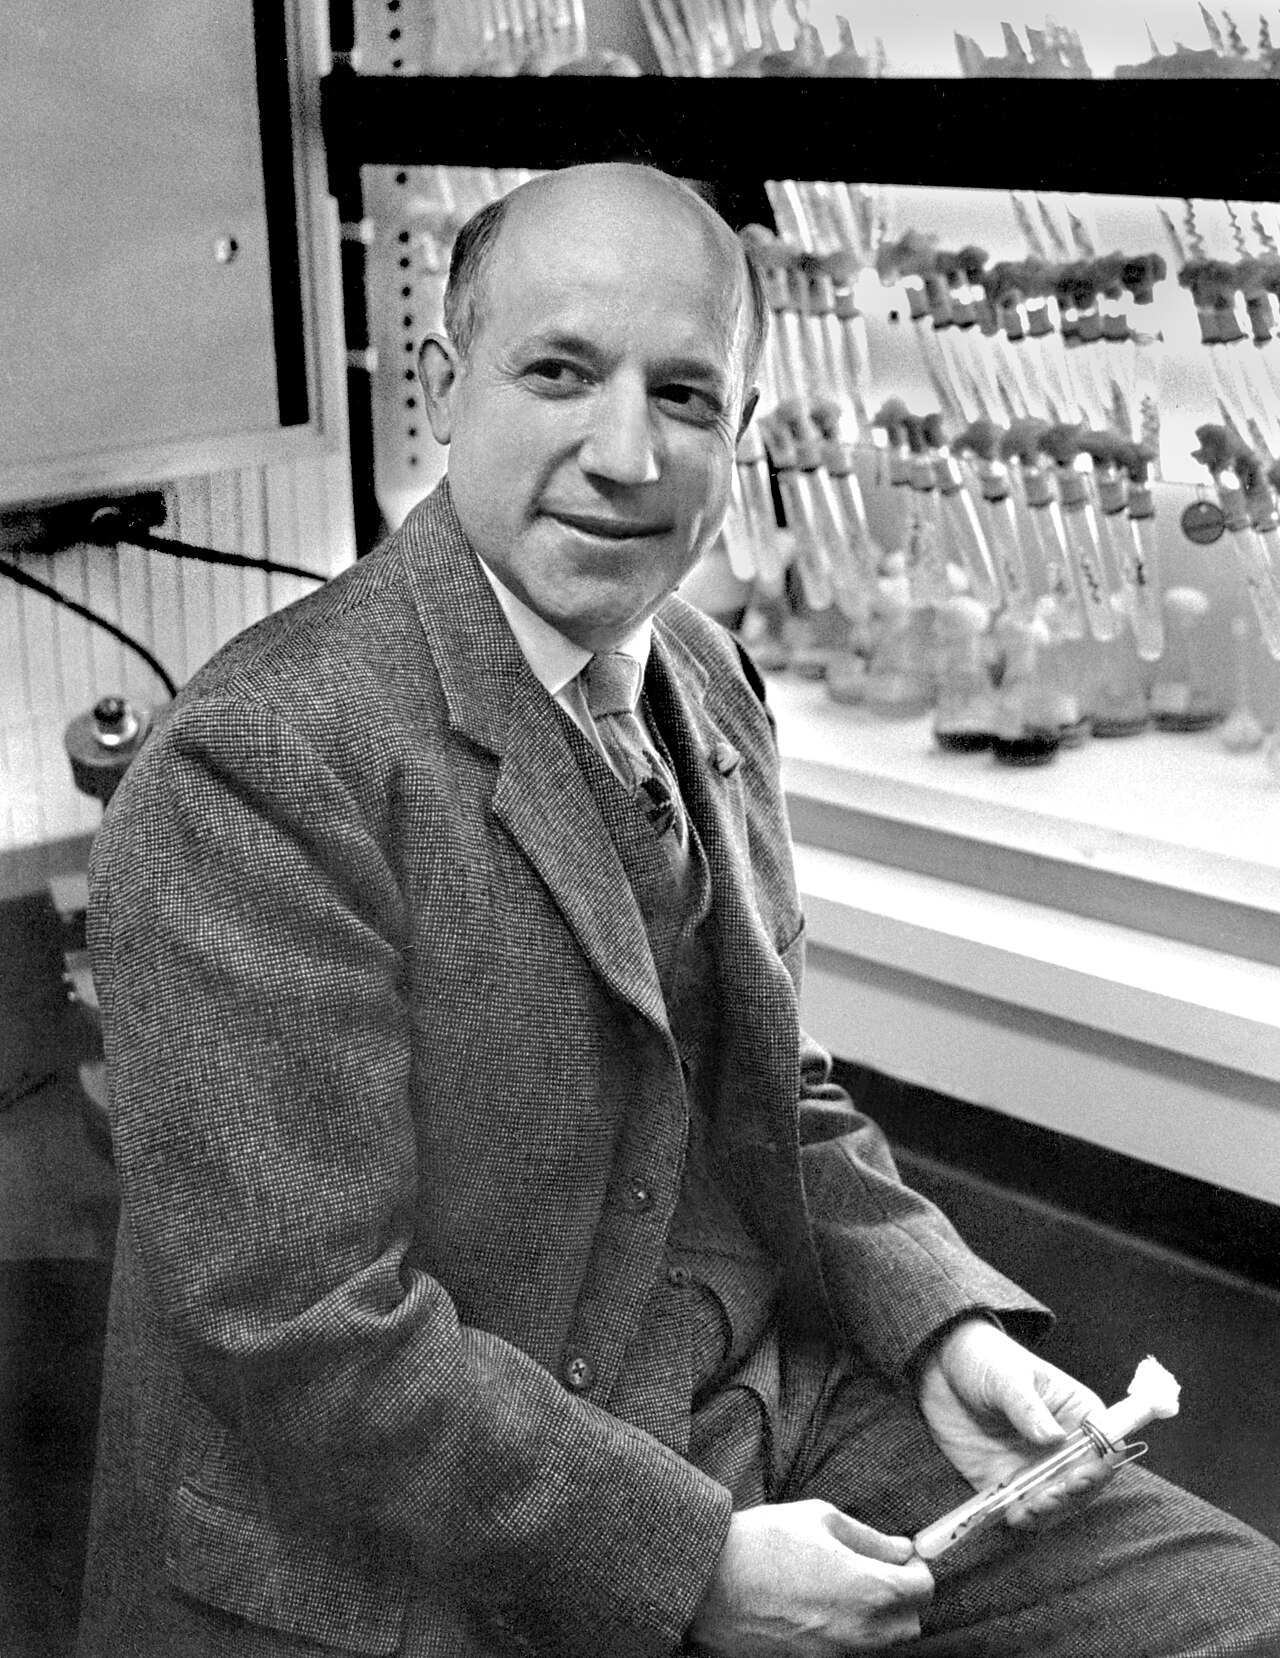
\includegraphics[width=0.26\linewidth]{images/book3/calvin.jpg}

{\small Melvin Calvin (1911--1997), que con Benson siguió el camino del
carbono desde el $\mathrm{CO_2}$ hasta el azúcar con carbono radiactivo y
cromatografía en papel. Fotografía: Lawrence Berkeley Laboratory, dominio
público.}
\end{omfigure}

\begin{omfigure}
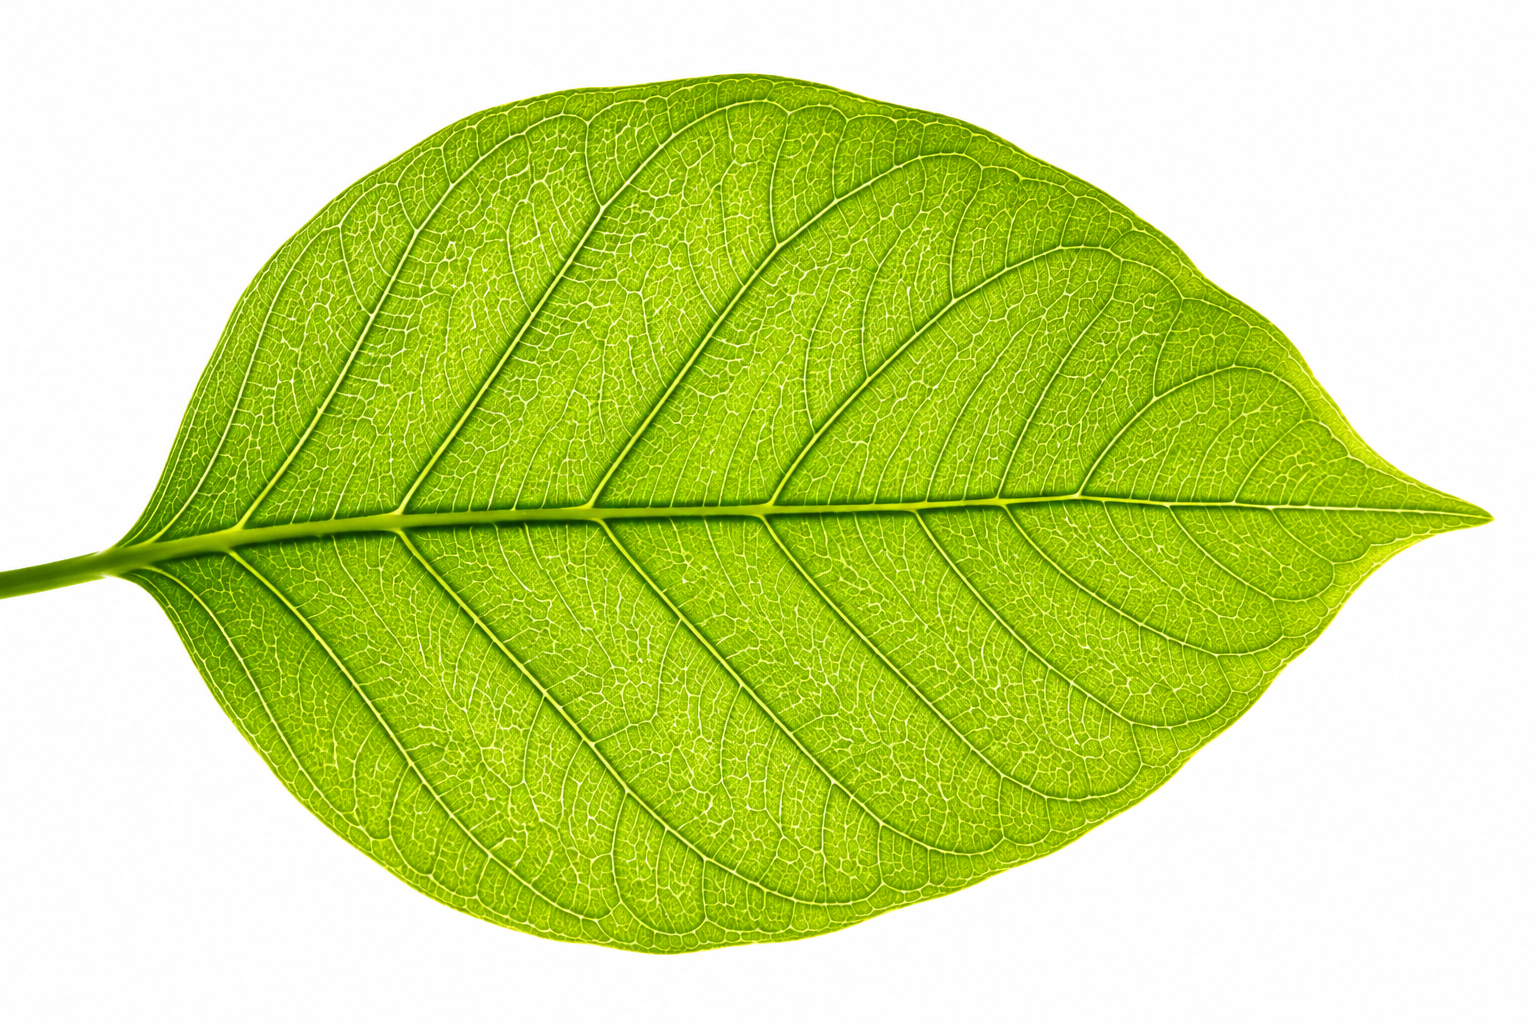
\includegraphics[width=0.6\linewidth]{images/book3/ai/b3-14-leaf-backlit.png}

{\small Una \omterm{def:b1:flowering-plant-organization:organs}{hoja} a contraluz: la luz que absorbe impulsa, en cada
\omterm{def:b1:photosynthesis:chloroplast}{cloroplasto} de sus \omterm{def:b1:cell-unit-of-life:cell}{células} en empalizada, la escisión del agua y la fijación
del dióxido de carbono que entró por sus \omterm{def:b1:flowering-plant-organization:tissues}{estomas}.}
\end{omfigure}

\begin{method}[Balance de un presupuesto fotosintético]\label{met:b1:photosynthesis:budget}
\begin{enumerate}
  \item Cuéntense los carbonos: cada $\mathrm{CO_2}$ fijado da un carbono de
        producto; una glucosa exige seis vueltas de la \omterm{def:b1:photosynthesis:fixation}{RuBisCO}.
  \item Cuéntense los transportadores: cada vuelta cuesta 3 \omterm{def:b1:water-small-molecules:atp}{ATP} y 2 NADPH
        (9 y 6 por G3P); una glucosa cuesta 18 \omterm{def:b1:water-small-molecules:atp}{ATP} y 12 NADPH.
  \item Cuéntense los fotones: el flujo lineal da 2 NADPH y unos 3 \omterm{def:b1:water-small-molecules:atp}{ATP} por
        $\mathrm{O_2}$, con 8 fotones (4 por \omterm{def:b1:photosynthesis:zscheme}{fotosistema}); 12 NADPH exigen
        6 $\mathrm{O_2}$ y 48 fotones; el \omterm{def:b1:water-small-molecules:atp}{ATP} adicional procede del flujo
        cíclico (unos cuantos fotones más). Unos 8 fotones por
        $\mathrm{CO_2}$: el requerimiento cuántico.
  \item Cuéntese la energía: un mol de fotones de \qty{680}{nm} son
        \qty{176}{kJ}; 48 fotones son \qty{8450}{kJ} para \qty{2870}{kJ}
        almacenados en glucosa: un \qty{34}{\%} como mucho, antes de
        cualquier pérdida por reflexión, respiración y por la fracción del
        espectro que no se absorbe.
\end{enumerate}
\end{method}

\section{Fotorrespiración, C4 y CAM}

\begin{proposition}[El defecto de la RuBisCO]\label{prop:b1:photosynthesis:photorespiration}
\index{fotorrespiración}
La \omterm{def:b1:photosynthesis:fixation}{RuBisCO} acepta también $\mathrm{O_2}$ en lugar de $\mathrm{CO_2}$: la
oxigenación de la RuBP rinde un 3-PGA y un fosfoglicolato de dos carbonos,
que la \omterm{def:b1:cell-unit-of-life:cell}{célula} debe recuperar por una ruta costosa a través de tres \omterm{def:b1:cell-unit-of-life:prokeuk}{orgánulos}
que libera $\mathrm{CO_2}$ y consume \omterm{def:b1:water-small-molecules:atp}{ATP}: la
\emph{fotorrespiración}. La \omterm{def:b1:enzymes:enzyme}{enzima} discrimina mal (unos \qty{80}{} a 1 a
favor del $\mathrm{CO_2}$ a igualdad de concentraciones), y en el aire el
$\mathrm{O_2}$ es quinientas veces más abundante que el $\mathrm{CO_2}$; a
\qty{25}{\celsius} se desperdicia la cuarta parte de las fijaciones, y más
con tiempo caluroso y seco, cuando los \omterm{def:b1:flowering-plant-organization:tissues}{estomas} se cierran y el
$\mathrm{CO_2}$ baja dentro de la \omterm{def:b1:flowering-plant-organization:organs}{hoja}. La \omterm{def:b1:photosynthesis:fixation}{RuBisCO}, que apareció cuando el
aire no tenía oxígeno, es además lenta (tres ciclos por segundo) y se
compensa con abundancia: es la \omterm{def:b1:proteins:peptide}{proteína} más abundante de la Tierra, la mitad
de la \omterm{def:b1:proteins:peptide}{proteína} soluble de una \omterm{def:b1:flowering-plant-organization:organs}{hoja}.
\end{proposition}

\begin{definition}[Plantas C4 y CAM]\label{def:b1:photosynthesis:c4cam}
\index{planta C4}\index{planta CAM}
Las \emph{plantas C4} (maíz, caña de azúcar, sorgo, muchas gramíneas
tropicales) cierran la fuga concentrando el $\mathrm{CO_2}$: en las \omterm{def:b1:cell-unit-of-life:cell}{células}
del mesófilo, una \omterm{def:b1:enzymes:enzyme}{enzima} sin afinidad por el $\mathrm{O_2}$ (la PEP
carboxilasa) fija el bicarbonato en un ácido de cuatro carbonos, que se
traslada a las \omterm{def:b1:cell-unit-of-life:cell}{células} de la \emph{vaina} que rodea los nervios y allí se
descarboxila, lo que multiplica por diez el $\mathrm{CO_2}$ en torno a la
\omterm{def:b1:photosynthesis:fixation}{RuBisCO} y suprime la oxigenación, a un coste de dos \omterm{def:b1:water-small-molecules:atp}{ATP} adicionales por
$\mathrm{CO_2}$. Los dos tipos celulares forman la anatomía \emph{Kranz}
(``corona''). Las \emph{plantas CAM} (cactus, piña, agaves) separan esos dos
mismos pasos en el tiempo y no en el espacio: abren sus \omterm{def:b1:flowering-plant-organization:tissues}{estomas} de noche,
almacenan el $\mathrm{CO_2}$ como ácido málico en la \omterm{def:b1:eukaryotic-cell:plantcell}{vacuola} y se lo liberan
de día a la \omterm{def:b1:photosynthesis:fixation}{RuBisCO} con los \omterm{def:b1:flowering-plant-organization:tissues}{estomas} cerrados, con lo que pierden la décima
parte del agua que pierde una planta C3 por carbono fijado.
\end{definition}

\begin{omfigure}
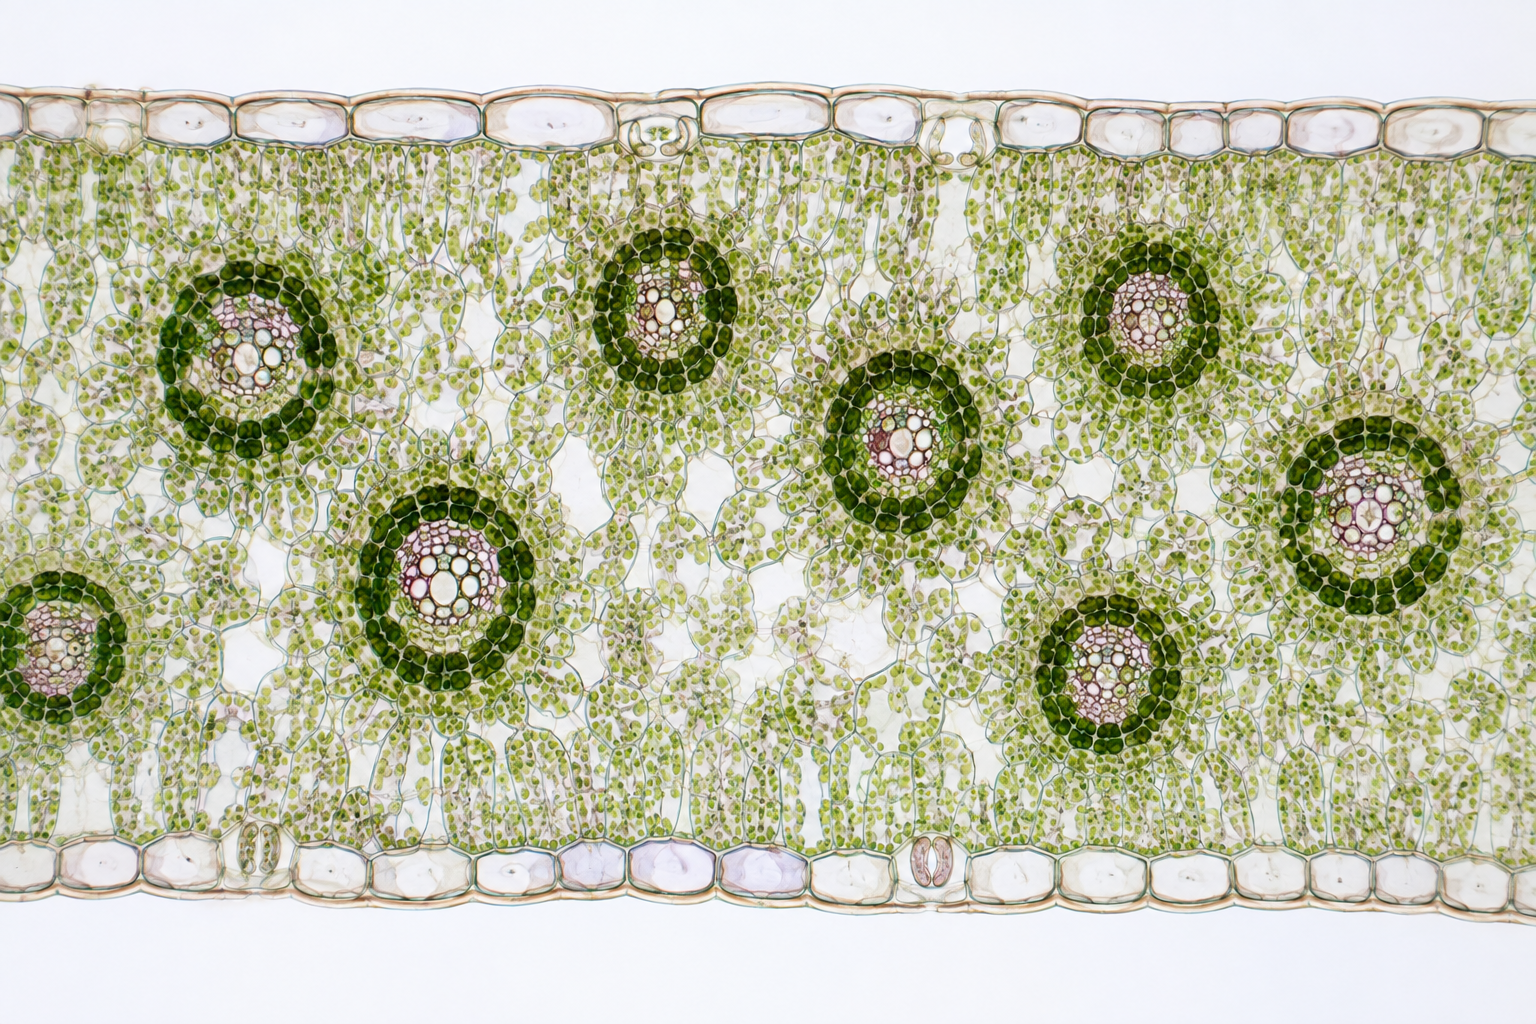
\includegraphics[width=0.6\linewidth]{images/book3/ai/b3-14-maize-kranz.png}

{\small Anatomía Kranz en una \omterm{def:b1:flowering-plant-organization:organs}{hoja} de maíz: cada nervio está coronado por
\omterm{def:b1:cell-unit-of-life:cell}{células} grandes de la vaina, repletas de \omterm{def:b1:eukaryotic-cell:plastid}{cloroplastos}, rodeadas a su vez por
\omterm{def:b1:cell-unit-of-life:cell}{células} del mesófilo. El $\mathrm{CO_2}$ se capta en el anillo exterior y se
entrega, concentrado, a la \omterm{def:b1:photosynthesis:fixation}{RuBisCO} del interior.}
\end{omfigure}

\begin{example}[Qué planta y dónde]\label{ex:b1:photosynthesis:where}
A \qty{20}{\celsius} y con aire húmedo, una \omterm{def:b1:flowering-plant-organization:organs}{hoja} C3 de trigo y una \omterm{def:b1:flowering-plant-organization:organs}{hoja} C4
de maíz fijan carbono a velocidades parecidas, y el maíz paga dos \omterm{def:b1:water-small-molecules:atp}{ATP} más
por carbono. A \qty{35}{\celsius} y con aire seco, el trigo pierde un tercio
de su fijación en fotorrespiración mientras que el maíz no pierde nada: las
gramíneas C4 dominan los campos abiertos y calurosos, y las plantas C3 los
lugares frescos y sombreados. Un cactus fija despacio según cualquiera de
los dos criterios, pero sobrevive donde los demás morirían de sed.
\end{example}

\section{Autotrofía}

\begin{definition}[Autotrofía]\label{def:b1:photosynthesis:autotrophy}
Un \omterm{def:b1:organism-environment:organism}{organismo} es \emph{autótrofo}\index{autotrofía} cuando construye su
materia orgánica a partir del $\mathrm{CO_2}$
(\cref{ch:b1:organism-environment}). Necesita una fuente de energía y una
fuente de electrones. Los \emph{\omterm{def:b1:organism-environment:trophy}{fotoautótrofos}} toman la energía de la luz:
las plantas, las algas y las cianobacterias toman sus electrones del agua y
liberan oxígeno (son \emph{oxigénicos}); las bacterias púrpuras y verdes los
toman del sulfuro de hidrógeno o de ácidos orgánicos y no liberan ninguno.
Los \emph{\omterm{def:b1:organism-environment:trophy}{quimioautótrofos}} toman tanto la energía como los electrones de la
oxidación de compuestos inorgánicos --- amoniaco, nitrito, sulfuro,
hidrógeno, hierro ferroso --- sin luz alguna: las bacterias nitrificantes
del suelo y las bacterias que alimentan los ecosistemas de las fuentes
hidrotermales. Todos usan el \omterm{def:b1:photosynthesis:fixation}{ciclo de Calvin}, o un ciclo emparentado, para
fijar el carbono; todos lo reducen con NADPH y lo pagan con \omterm{def:b1:water-small-molecules:atp}{ATP}; solo
difieren en de dónde vienen el \omterm{def:b1:water-small-molecules:atp}{ATP} y los electrones.
\end{definition}

\begin{example}[El balance global]\label{ex:b1:photosynthesis:global}
La fotosíntesis fija unas \qty{120}{Gt} de carbono al año en tierra firme y
\qty{50}{Gt} en los océanos, la mitad de ellas por algas unicelulares y
cianobacterias invisibles a la vista; renueva el dióxido de carbono de la
atmósfera cada siete años y su oxígeno cada dos mil. El oxígeno llegó por la
misma vía: durante dos mil millones de años las cianobacterias lo liberaron
a una atmósfera que no lo tenía, y todo \omterm{def:b1:organism-environment:organism}{organismo} aerobio, desde la
\omterm{def:b1:eukaryotic-cell:mitochondrion}{mitocondria} hacia arriba, está construido sobre la fuga de un sistema
enzimático que escinde el agua.
\end{example}

\section{Ejercicios}

\begin{exercise}[$\star$]\label{exo:b1:photosynthesis:1}
Nómbrense los tres sistemas de membranas del \omterm{def:b1:photosynthesis:chloroplast}{cloroplasto} y dígase dónde
ocurren las \omterm{prop:b1:photosynthesis:lightreactions}{reacciones luminosas} y el \omterm{def:b1:photosynthesis:fixation}{ciclo de Calvin}.
\end{exercise}

\begin{exercise}[$\star$]\label{exo:b1:photosynthesis:2}
Escríbase la ecuación de las \omterm{prop:b1:photosynthesis:lightreactions}{reacciones luminosas} y dígase de dónde procede
el oxígeno liberado, con las pruebas correspondientes.
\end{exercise}

\begin{exercise}[$\star$]\label{exo:b1:photosynthesis:3}
Nómbrense las tres etapas del \omterm{def:b1:photosynthesis:fixation}{ciclo de Calvin} y el número de \omterm{def:b1:water-small-molecules:atp}{ATP} y de NADPH
consumidos por cada $\mathrm{CO_2}$ fijado.
\end{exercise}

\begin{exercise}[$\star$]\label{exo:b1:photosynthesis:4}
A partir de la figura de los espectros, ¿a qué longitudes de onda absorbe
más la \omterm{def:b1:photosynthesis:pigments}{clorofila} $a$, y por qué el espectro de acción es más alto que la
absorción de la \omterm{def:b1:photosynthesis:pigments}{clorofila} en torno a \qty{500}{nm}?
\end{exercise}

\begin{exercise}[$\star\star$]\label{exo:b1:photosynthesis:5}
Explíquense el efecto de aumento de Emerson y qué reveló sobre la
organización de las \omterm{prop:b1:photosynthesis:lightreactions}{reacciones luminosas}.
\end{exercise}

\begin{exercise}[$\star\star$]\label{exo:b1:photosynthesis:6}
¿A cuánta \omterm{prop:b1:water-small-molecules:gibbs}{energía libre} por mol de protones corresponde una fuerza
protón-motriz de \qty{0.18}{V} ($F = \qty{96500}{C/mol}$)? ¿Cuántos protones
deben fluir para fabricar un \omterm{def:b1:water-small-molecules:atp}{ATP} de \qty{50}{kJ/mol}? Compárese con los
cuatro que usa la sintasa.
\end{exercise}

\begin{exercise}[$\star\star$]\label{exo:b1:photosynthesis:7}
Los \omterm{def:b1:photosynthesis:chloroplast}{tilacoides} de Jagendorf fabricaron \omterm{def:b1:water-small-molecules:atp}{ATP} en la oscuridad tras un baño
ácido. Explíquese qué demuestra esto y qué no, y predígase el resultado si
se añade un desacoplante antes de la transferencia.
\end{exercise}

\begin{exercise}[$\star\star$]\label{exo:b1:photosynthesis:8}
Sígase el carbono: partiendo de 3 RuBP (15 carbonos) y 3 $\mathrm{CO_2}$,
cuéntense los carbonos a través del 3-PGA, del G3P, del G3P exportado y de
la RuBP regenerada, y compruébese el balance.
\end{exercise}

\begin{exercise}[$\star\star$]\label{exo:b1:photosynthesis:9}
En el experimento de Calvin, la RuBP sube y el 3-PGA baja cuando se retira
el $\mathrm{CO_2}$; el 3-PGA sube y la RuBP baja cuando se apaga la luz.
Explíquense ambas cosas a partir del ciclo.
\end{exercise}

\begin{exercise}[$\star\star\star$]\label{exo:b1:photosynthesis:10}
Calcúlense la energía de un mol de fotones de \qty{680}{nm}
($h =
\qty{6.63e-34}{J.s}$, $c = \qty{3.0e8}{m/s}$, $N_A = \num{6.02e23}$),
la energía de los 48 fotones necesarios por glucosa y el rendimiento de
almacenar \qty{2870}{kJ/mol}. ¿Por qué el rendimiento de todo un cultivo,
alrededor del \qty{1}{\%} de la luz solar, es tanto menor?
\end{exercise}

\begin{exercise}[$\star\star\star$]\label{exo:b1:photosynthesis:11}
A \qty{25}{\celsius} y en aire, la \omterm{def:b1:photosynthesis:fixation}{RuBisCO} oxigena una vez por cada tres
carboxilaciones; cada oxigenación libera medio $\mathrm{CO_2}$ en el rescate
y cuesta \omterm{def:b1:water-small-molecules:atp}{ATP}. Calcúlense el carbono neto fijado por cada 100
carboxilaciones y la fracción perdida. Una \omterm{def:b1:photosynthesis:c4cam}{planta C4} evita la pérdida pero
gasta 2 \omterm{def:b1:water-small-molecules:atp}{ATP} adicionales por $\mathrm{CO_2}$: ¿a partir de qué fracción de
pérdida sale a cuenta el diseño C4, si un \omterm{def:b1:water-small-molecules:atp}{ATP} vale aproximadamente la décima
parte de un $\mathrm{CO_2}$ fijado?
\end{exercise}

\begin{exercise}[$\star\star\star$]\label{exo:b1:photosynthesis:12}
``La fotosíntesis es la respiración al revés.'' Discútase en un párrafo,
comparando el mecanismo quimiosmótico, el sentido del flujo de electrones,
los transportadores y los ciclos, y diciendo dónde se sostiene la analogía y
dónde falla.
\end{exercise}

\section{Problema: el precio de una molécula de glucosa}

\begin{problem}[{Problema de fin de semana --- fotones contados, electrones
y protones seguidos a través del tilacoide, ATP y NADPH calculados y
gastados, la cosecha diaria de una hoja pesada, hasta llegar al rendimiento
energético de la fotosíntesis}]
\label{pb:b1:photosynthesis:1}
Constantes: $h = \qty{6.63e-34}{J.s}$, $c = \qty{3.00e8}{m/s}$,
$N_A = \num{6.02e23}$, $F = \qty{96500}{C/mol}$, $R = \qty{8.314}{J.mol^{-1}.K^{-1}}$,
$T = \qty{298}{K}$. \omterm{prop:b1:water-small-molecules:gibbs}{Energía libre} de combustión de la glucosa,
\qty{2870}{kJ/mol}; la síntesis de \omterm{def:b1:water-small-molecules:atp}{ATP} en el \omterm{def:b1:photosynthesis:chloroplast}{cloroplasto} cuesta
\qty{50}{kJ/mol}; el NADPH contiene \qty{220}{kJ/mol} de poder reductor.

\medskip
\noindent\textbf{Parte I --- Fotones y electrones.}
\begin{enumerate}
  \item Calcúlense la energía de un fotón de \qty{680}{nm} y la de un mol
        de ellos.
  \item Calcúlense la energía de un mol de fotones de \qty{700}{nm} y la de
        uno de \qty{450}{nm}. ¿Por qué la luz azul no da más fotosíntesis
        por fotón que la roja?
  \item ¿Cuántos fotones de \qty{680}{nm} transportan un julio?
  \item Llevar un electrón desde el agua ($E'_0 = \qty{+0.82}{V}$) hasta el
        $\mathrm{NADP^+}$ ($E'_0 = \qty{-0.32}{V}$), ¿cuánta \omterm{prop:b1:water-small-molecules:gibbs}{energía libre}
        exige por mol de electrones ($\Delta G = -nF\Delta E$)?
  \item Se usan dos fotones por electrón (uno en cada \omterm{def:b1:photosynthesis:zscheme}{fotosistema}).
        Calcúlense la energía aportada por mol de electrones y la fracción
        de ella almacenada en el cambio redox.
  \item ¿Cuántos electrones, y por tanto cuántos fotones, hacen falta para
        fabricar un $\mathrm{O_2}$ y dos NADPH?
  \item ¿Cuántos fotones por glucosa, si hacen falta 12 NADPH?
\end{enumerate}

\medskip
\noindent\textbf{Parte II --- Protones y \omterm{def:b1:water-small-molecules:atp}{ATP}.}
Por cada $\mathrm{O_2}$ liberado se liberan cuatro protones en la luz
tilacoidal al escindirse el agua y el complejo citocromo $b_6f$ bombea ocho;
la \omterm{thm:b1:photosynthesis:chemiosmosis}{ATP sintasa} usa \qty{4}{H^+} por \omterm{def:b1:water-small-molecules:atp}{ATP}. La luz tilacoidal está a pH 5 y el
\omterm{def:b1:photosynthesis:chloroplast}{estroma} a pH 8; el \omterm{def:b1:membranes-transport:potential}{potencial de membrana} a través del \omterm{def:b1:photosynthesis:chloroplast}{tilacoide} es
despreciable.
\begin{enumerate}[resume]
  \item Calcúlense la fuerza protón-motriz a partir de la diferencia de pH,
        en voltios ($\Delta\mu = 2.303\,RT\,\Delta\mathrm{pH}/F$), y la
        \omterm{prop:b1:water-small-molecules:gibbs}{energía libre} por mol de protones.
  \item Calcúlense los protones entregados a la luz tilacoidal por
        $\mathrm{O_2}$ y el \omterm{def:b1:water-small-molecules:atp}{ATP} que pueden fabricar.
  \item Calcúlese el \omterm{def:b1:water-small-molecules:atp}{ATP} fabricado por glucosa mediante el flujo lineal (6
        $\mathrm{O_2}$), y compárese con los 18 que necesita el \omterm{def:b1:photosynthesis:fixation}{ciclo de
        Calvin}. ¿Cómo se cubre el déficit?
  \item Calcúlense la \omterm{prop:b1:water-small-molecules:gibbs}{energía libre} disponible de los protones por \omterm{def:b1:water-small-molecules:atp}{ATP}
        (\qty{4}{H^+}) y el rendimiento de la sintasa.
  \item La luz tilacoidal de un \omterm{def:b1:photosynthesis:chloroplast}{cloroplasto} tiene un volumen de unos
        \qty{1}{\micro m^3}. ¿Cuántos protones libres contiene a pH 5?
        Compárese con los aproximadamente $10^5$ protones que atraviesan
        las sintasas cada segundo, y conclúyase qué tampona esa luz.
\end{enumerate}

\medskip
\noindent\textbf{Parte III --- Azúcar.}
\begin{enumerate}[resume]
  \item Escríbase la energía almacenada por glucosa como 18 \omterm{def:b1:water-small-molecules:atp}{ATP} $\times$
        \qty{50}{kJ} más 12 NADPH $\times$ \qty{220}{kJ}, y compárese con
        los \qty{2870}{kJ} de la glucosa. ¿A dónde va la diferencia?
  \item Calcúlense la energía de los 48 fotones de la pregunta 6 y el
        rendimiento de la fotosíntesis desde el fotón hasta la glucosa.
  \item Solo el \qty{45}{\%} de la luz solar está en las longitudes de onda
        que absorben los pigmentos, y de ella una décima parte se refleja o
        se transmite. Calcúlese el rendimiento desde la luz solar incidente
        hasta la glucosa, antes de la respiración.
  \item Una \omterm{def:b1:flowering-plant-organization:organs}{hoja} de \qty{50}{cm^2} recibe \qty{400}{W/m^2} de luz solar
        durante \qty{10}{h}. Calcúlense la energía recibida y, con el
        rendimiento de la pregunta 14, la glucosa fabricada en gramos
        (\qty{180}{g/mol}).
  \item La \omterm{def:b1:flowering-plant-organization:organs}{hoja} respira el \qty{40}{\%} de esa glucosa para mantenerse
        viva. ¿Cuál es su ganancia neta, en gramos de glucosa y en gramos
        de carbono?
  \item Un cultivo alcanza un \qty{1}{\%} de rendimiento global en una
        temporada. Enumérense tres pérdidas, además de las ya contadas, que
        separen la cifra de la \omterm{def:b1:flowering-plant-organization:organs}{hoja} de la del cultivo.
\end{enumerate}

\medskip
\noindent\textbf{Parte IV --- La fuga.}
La \omterm{def:b1:photosynthesis:fixation}{RuBisCO} en aire a \qty{25}{\celsius} realiza una oxigenación por cada
tres carboxilaciones; cada oxigenación cuesta el equivalente de medio
$\mathrm{CO_2}$ fijado y 3,5 \omterm{def:b1:water-small-molecules:atp}{ATP}.
\begin{enumerate}[resume]
  \item Por cada 100 carboxilaciones, calcúlense las oxigenaciones, el
        carbono perdido y el carbono neto ganado.
  \item Calcúlense el \omterm{def:b1:water-small-molecules:atp}{ATP} gastado en el rescate por cada 100
        carboxilaciones y el \omterm{def:b1:water-small-molecules:atp}{ATP} total por carbono neto ganado (3 \omterm{def:b1:water-small-molecules:atp}{ATP} del
        \omterm{def:b1:photosynthesis:fixation}{ciclo de Calvin} por carboxilación más el rescate).
  \item Una \omterm{def:b1:photosynthesis:c4cam}{planta C4} no oxigena, pero gasta 2 \omterm{def:b1:water-small-molecules:atp}{ATP} adicionales por
        $\mathrm{CO_2}$ entregado. Calcúlese su \omterm{def:b1:water-small-molecules:atp}{ATP} por carbono neto y
        compárese.
  \item A \qty{35}{\celsius} la proporción de oxigenaciones sube a una de
        cada dos. Recalcúlense las cifras de la C3 y dígase qué diseño
        gana.
  \item Explíquese por qué elevar el $\mathrm{CO_2}$ de un invernadero al
        triple del valor atmosférico aumenta el rendimiento de los cultivos
        C3 (tomate, trigo) pero apenas el de los C4 (maíz).
  \item Una \omterm{def:b1:flowering-plant-organization:organs}{hoja} C3 pierde unas 250 moléculas de agua por cada
        $\mathrm{CO_2}$ fijado, y una \omterm{def:b1:photosynthesis:c4cam}{planta CAM} unas 25. Calcúlese el agua
        que pierde cada una para fijar \qty{1}{g} de carbono.
  \item Enúnciese el resultado: el requerimiento cuántico por
        $\mathrm{CO_2}$, el rendimiento desde el fotón hasta la glucosa y
        el rendimiento desde la luz solar hasta el azúcar neto de la \omterm{def:b1:flowering-plant-organization:organs}{hoja}.
\end{enumerate}
\end{problem}
